% Escolha: Portugues ou Ingles ou Espanhol.
% Para a versão final do texto, após a defesa, acrescente Final:

\documentclass[Portugues]{phdquali}
%\documentclass[Portugues,Final]{phdquali}

\usepackage[latin1,utf8]{inputenc}

% Para identar primeiro parágrafo:
\usepackage{indentfirst}

% Para transformar caption em negrito:
\usepackage[font=footnotesize,labelfont=bf]{caption}

% Para trocar o estilo dos hyperlinks:
\usepackage{hyperref}
\hypersetup{
  colorlinks   = true, % Colours links instead of ugly boxes
  urlcolor     = blue, % Colour for external hyperlinks
  linkcolor    = black, % Colour of internal links
  citecolor   = black % Colour of citations
}

% Letras gregas (alfa, beta, gamma, etc) em modo texto:
\usepackage{textgreek} % \textalpha, \textbeta, \textgamma, etc

% Para usar letras no enumerate:
\usepackage{enumitem}

% Formatar \listoffigures
\usepackage{tocloft}
\renewcommand{\cftfigpresnum}{Figure }
\renewcommand{\cftfignumwidth}{6em}

% % Para acrescentar comentários ao PDF descomente:
% \usepackage
% %  [pdfauthor={nome do autor},
% %   pdftitle={titulo},
% %   pdfkeywords={palavra-chave, palavra-chave},
% %   pdfproducer={Latex with hyperref},
% %   pdfcreator={pdflatex}]
% {hyperref}

% Define atalhos
\def\ie{i.e.\onedot} 
\def\Ie{I.e.\onedot}
\def\eg{e.g.\onedot}
\def\Eg{E.g.\onedot}

\begin{document}

% Escolha entre autor ou autora:
\autor{João Victor da Silva Guerra}
%\autora{Nome da Autora}

% Sempre deve haver um título em português:
\titulo{Desenvolvimento de plataforma de metodologias computacionais para caracterização estrutural e funcional de biomoléculas e sítios de ligação}

% Se a língua for o inglês ou o espanhol defina:
%\title{The Dissertation or Thesis Title in English or Spanish}

% Escolha entre orientador ou orientadora. Inclua os títulos acadêmicos:
\orientador{Prof. Dr. Paulo Sergio Lopes-de-Oliveira}
%\orientadora{Profa. Dra. Nome da Orientadora}

% Escolha entre coorientador ou coorientadora, se houver.  Inclua os títulos acadêmicos:
%\coorientador{Prof. Dr. Eng. Lic. Nome do Co-Orientador}
%\coorientadora{Profa. Dra. Eng. Lic. Nome da Co-Orientadora}

% Escolha entre mestrado ou doutorado:
% \mestrado
\doutorado

% Se houve cotutela, defina:
%\cotutela{Universidade Nova de Plutão}

\datadadefesa{01}{01}{2023}

% Para a versão final defina:
%\avaliadorA{Prof. Dr. Primeiro Avaliador}{Instituição do primeiro avaliador}
%\avaliadorB{Profa. Dra. Segunda Avaliadora}{Instituição da segunda avaliadora}
%\avaliadorC{Dr. Terceiro Avaliador}{Instituição do terceiro avaliador}
%\avaliadorD{Prof. Dr. Quarto Avaliador}{Instituição do quarto avaliador}
%\avaliadorE{Prof. Dr. Quinto Avaliador}{Instituição do quinto avaliador}
%\avaliadorF{Prof. Dr. Sexto Avaliador}{Instituição do sexto avaliador}
%\avaliadorG{Prof. Dr. Sétimo Avaliador}{Instituição do sétimo avaliador}
%\avaliadorH{Prof. Dr. Oitavo Avaliador}{Instituição do oitavo avaliador}


% Para incluir a ficha catalográfica em PDF na versão final, descomente e ajuste:
%\fichacatalografica{arquivo.pdf}


% Este comando deve ficar aqui:
\paginasiniciais


% Se houver dedicatória, descomente:
%\prefacesection{Dedicatória}
%A dedicatória deve ocupar uma única página.


% Se houver epígrafe, descomente e edite:
% \begin{epigrafe}
% {\it
% Vita brevis,\\
% ars longa,\\
% occasio praeceps,\\
% experimentum periculosum,\\
% iudicium difficile.}
%
% \hfill (Hippocrates)
% \end{epigrafe}


% Agradecimentos ou Acknowledgements ou Agradecimientos
\prefacesection{Agradecimentos}

Gostaria de expressar meus sinceros agradecimentos a todos que me apoiaram durante o desenvolvimento deste projeto. Em primeiro lugar, sou grato aos meus pais, Roseli do Carmo Freitas da Silva e Mario Luiz da Silva Guerra, por me apoiarem em todas as etapas da minha formação acadêmica e profissional. Agradeço à minha companheira, Bruna Martins da Silva, pelo apoio incondicional em todas as fases deste projeto.

Gostaria de agradecer ao meu orientador, Dr. Paulo Sergio Lopes de Oliveira, por ter me dado liberdade científica e criativa para desenvolver esta tese e, acima de tudo, pela oportunidade de trabalhar em um centro de pesquisa de excelência. Agradeço aos meus colegas do Laboratório de Biologia Computacional, José Geraldo de Carvalho Pereira, Helder Veras Ribeiro Filho, Luiz Fernando Giolo Alves, Mariana Bortoletto Grizante, Gabriel Ernesto Jara e Leandro Oliveira Bortot, por terem me apoiado em momentos importantes, compartilhando ideias e sugestões para o desenvolvimento deste projeto. Sou imensamente grato a todos que me ajudaram nesta etapa essencial da minha formação acadêmica.

Por fim, gostaria de agradecer ao Programa de Pós-Graduação em Ciências Farmacêuticas da Faculdade de Ciências Farmacêuticas da Universidade Estadual de Campinas, ao Laboratório Nacional de Biociências e ao Centro Nacional de Pesquisa em Energia e Materiais, por terem viabilizado este trabalho. Também sou grato pelo apoio financeiro da Fundação de Amparo à Pesquisa do Estado de São Paulo (FAPESP) pelo projeto de pesquisa regular (processo nº 2018/00629-0, Fundação de Amparo à Pesquisa do Estado de São Paulo (FAPESP))."


% Sempre deve haver um resumo em português:
\begin{resumo}
O resumo deve ter no máximo 500 palavras e deve ocupar uma única página.
\end{resumo}


% Sempre deve haver um abstract:
\begin{abstract}
The abstract must have at most 500 words and must fit in a single page.
\end{abstract}


% Se houver um resumo em espanhol, descomente:
%\begin{resumen}
% A mesma regra aplica-se.
%\end{resumen}


% A lista de figuras é opcional:
\listoffigures
\clearpage

% A lista de tabelas é opcional:
\listoftables
\clearpage

% A lista de abreviações e siglas é opcional:
\prefacesection{Lista de Abreviações e Siglas}

\begin{itemize}
  \item[3D] Tridimensional
  \item[GHECOM] \textit{Grid-based HECOMi finder}
  \item[IPD] Interações Proteína-DNA
  \item[IPL] Interações Proteína-Ligante
  \item[IPR] Interações Proteína-RNA
  \item[IPP] Interações Proteína-Proteína
  \item[KVFinderMD] \textit{KVFinder for Molecular Dynamics analysis}
  \item[LES] Superfície Excluída pelo Ligante (\textit{Ligand Excluded Surface})
  \item[parKVFinder] \textit{Parallel KVFinder}
  \item[Pi] \textit{Probe In}
  \item[Po] \textit{Probe Out}
  \item[pyKVFinder] \textit{Python-C Parallel KVFinder}
  \item[SAS] Superfície Acessível ao Solvente (\textit{Solvent Accessible Surface})
  \item[SES] Superfície Excluída pelo Solvente (\textit{Solvent Excluded Surface})
  \item[vdW] van der Waals
  \item[wwPDB] Worldwide Protein Data Bank
\end{itemize}

\clearpage

% A lista de símbolos é opcional:
% \prefacesection{Lista de Símbolos}

% Quem usa o pacote nomencl pode incluir:
% \renewcommand{\nomname}{Lista de Abreviações e Siglas}
% \printnomenclature[3cm]


% O sumário vem aqui:
\tableofcontents


% E esta linha deve ficar bem aqui:
\fimdaspaginasiniciais

% O corpo da dissertação ou tese começa aqui:

%%% Chapter 1

\chapter{Introdução}

% \begin{itemize}
%  \item Comece explicando a importância dos sítios de ligação em biomoléculas e como eles afetam a função biológica das moléculas;
%  \item Apresente os métodos experimentais e computacionais disponíveis para identificar e caracterizar sítios de ligação;
%  \item Descreva brevemente os programas computacionais mais utilizados na área e suas principais características;
%  \item Finalize apresentando o objetivo e a estrutura do seu trabalho.
% \end{itemize}

Biomoléculas, como proteínas e ácidos núcleios, são moléculas complexas que desempenham funções biológicas essenciais para a vida. Processos biológicos, como a transdução de sinal, a integridade estrutural, a adesão celular e a apoptose, são modulados por interações biomoleculares \cite{sotriffer2002,henrich2010}. Essas interações são extremamente importantes para a compreensão de processo biológicos e para o desenvolvimento e/ou aprimoramento de terapias farmacológicas \cite{henrich2010}. No entanto, os estudos dos mecanismos intrínsicos dessas interações ou possíveis pontos de interação são desafiadores, devido à complexidade das biomoléculas e à diversidade das interações que ocorrem entre elas.

Usualmente, essas interações ocorrem entre os receptores e ligantes, que variam de íons, como ferro e fosfato, a macromoléculas, como proteínas, RNA e DNA \cite{oliveira2014}. Para execução dessas interações, estruturas atomísticas se dobram orquestradamente para criar sítios de ligação específicos, comumente localizados em cavidades ao longo da superfície molecular, expondo padrões topológicos e físico-químicos para acomodar ligantes específicos \cite{henrich2010,guerra2021}. As interações receptor-ligante, como interações proteína-proteína (IPP), proteína-ligante (IPL), proteína-RNA (IPR) e proteína-DNA (IPD), são consequência da complementariedade entre as superfícies moleculares do par de interação, restringindo assim a um pequeno número de ligantes a interação eficiente com um dado receptor \cite{henrich2010,simoes2017}.

Dada a importância das interações biomoleculares, o estudo das biomoléculas e seus sítios de ligação são essencias para compreensão de processos biológicos e para o aprimoramento e desenvolvimento de novos fármacos. A utilização de abordagens computacionais para identificar sítios de ligação e caracterizar interações biomoleculares tem se mostrado uma alternativa eficaz para complementar os métodos experimentais e fornecer informações detalhadas sobre as interações moleculares \cite{simoes2017}. A identificação de sítios de ligação é um problema de classificação, onde o objetivo é determinar se um dado ponto na superfície de uma biomolécula é um sítio de ligação ou não \cite{sotriffer2002,henrich2010,simoes2017}. Enquanto isso, avanços em recursos computacionais e base de dados têm impulsionado o uso de métodos \textit{in silico} para simular a dinâmica de biomoléculas e implementar aplicações de inteligência artificial para estudar estruturas biomoleculares \cite{tunyasuvunakool2021}. Juntos, todos esses dados estruturais fornecem terreno fértil para interpretação de dados por meio de ciência de dados ou protocolos automatizadas, mas a análise intensiva de dados requer rotinas eficientes e integráveis com uma estrutura de dados facilmente manipulável.

Nesse cenário, ainda há a necessidade de ferramentas computacionais robustas e abrangentes para estudos computacionais de sistemas biomoleculares, capazes de cobrir as diferentes formas de interação. Ferramentas que sirvam como blocos de construção, para aplicações, programas e/ou protocolos automatizados de biologia computacional, biologia estrutural, aprendizado de máquina e áreas correlatas, são essenciais para análise de biomoléculas e/ou sítios de ligação. O desenvolvimento de ferramentas que possam ser utilizadas em diferentes tipos de aplicações e potencialidades é de suma importância nesse contexto.

Nesse sentido, o KVFinder suite é uma plataforma computacional que tem como objetivo atender a essas demandas. O KVFinder suite é composto por um conjunto de ferramentas para codificação e caracterização de biomoléculas e detecção e caracterização de sítios de ligação nessas biomoléculas. O KVFinder suite é composto por cinco ferramentas: parKVFinder \cite{guerra2020}, pyKVFinder \cite{guerra2021}, KVFinder-web \cite{guerra2023A}, KVFinderMD e SERD. Essa plataforma tem o potencial de ser uma ferramenta robusta e abrangente para estudos computacionais de sistemas biomoleculares, e pode ser utilizada em diferentes aplicações e contextos, desde a biologia estrutural até a ciência de dados.


\section{Identificação de sítios de ligação em biomoléculas \label{sec:binding-sites}}

Ao longo das últimas décadas, diversas abordagens \textit{in silico} foram desenvolvidas para identificação de sítios de ligação em proteínas para aprofundar os conhecimentos acerca de função de uma determinada proteína e para descoberta e melhoramento de fármacos \cite{liang1998}. No entanto, apenas algumas metodologias são aplicáveis à outros tipos de biomoléculas, \eg, ácidos núcleicos, carboidratos e lípideos. As abordagens computacionais publicados podem ser divididos em três categorias principais: geométricas, energéticas e evolutivas \cite{oliveira2014,simoes2017}.

\begin{itemize}
  \item \textbf{Métodos evolutivos:} são baseados na busca por resíduos conservados em alinhamentos de sequências múltiplas e informações de perfis conhecidos de sítios de ligação;
  \item \textbf{Métodos energéticos:} identificam sítios de ligação a partir da interação energética entre a biomolécula-alvo e uma sonda química, geralmente um grupo químico;
  \item \textbf{Métodos geométricos:} identificam cavidades analisando as características geométricas da superfície molecular.
\end{itemize}

Cada categoria de métodos possui suas próprias vantagens e desvantagens \cite{sotriffer2002,henrich2010,simoes2017,krone2016}. Algoritmos evolutivos dependem fortemente de informações de sequência ou bancos de dados de sítios de ligação ativos e da qualidade do procedimento de alinhamento, enquanto os métodos energéticos dependem de procedimentos de filtragem, parametrizações de campo de força e funções de pontuação utilizadas. Por outro lado, métodos de detecção geométrica são relativamente simples e diretos e não exigem nenhum conhecimento não geométrico, apenas dados estruturais da proteína, \ie o arquivo no formato PDB, XYZ, mmCIF ou equivalente, contendo as coordenadas cartesianas dos átomos, que podem ser facilmente acessadas no Worldwide Protein Data Bank (wwPDB). Uma vez que as coordenadas dos átomos estão disponíveis, métodos geométricos devem ser capazes de representar qualquer tipo de biomolécula. \cite{henrich2010,oliveira2014,simoes2017}. Embora métodos puramente geométricos sejam eficientes na identificação de todos os tipos de cavidades de uma molécula alvo, identificar aquelas que são funcionalmente relevantes apresenta um problema. No entanto, a caracterização de cavidades em termos de propriedades físico-químicas bem escolhidas pode levar à identificação de cavidades funcionalmente relevantes, ou seja, sítios de ligação para um conjunto específico de ligantes \cite{sotriffer2002,henrich2010,simoes2017,liang1998}.

Em geral, algoritmos baseados em geometria são os mais frequentemente usados para detectar cavidades em proteínas. Enquanto métodos baseados em evolução seriam limitados a proteínas porque dependem de princípios da evolução biológica, métodos baseados em energia poderiam ser aplicáveis, mas exigiriam ajustes finos dos parâmetros de campo de força adaptados à outros tipos de biomoléculas. Como ácidos núcleicos, carboidratos e lipídeos podem ter propriedades distintas em comparação com proteínas, métodos que dependem apenas de informações geométricas (por exemplo, coordenadas Cartesianas tridimensionais (3D) e tamanho do átomo) são desejáveis.

\subsection{Abordagens geométricas \label{sec:geometric-approaches}}

A detecção de cavidades através de abordagens geométricas é amplamente utilizada, envolvendo diferentes técnicas \cite{simoes2017,guerra2020,krone2016}. Essas técnicas são simples, diretas e não requerem conhecimento prévio, tornando-as as mais comumente utilizadas na literatura \cite{henrich2010,oliveira2014}. Neste contexto, apresentamos uma breve classificação abrangente das abordagens geométricas para detecção de cavidades, incluindo técnicas baseadas em grade 3D, sonda, tesselação, superfície e suas combinações \cite{simoes2017,guerra2020,krone2016,guerra2023B}.

\begin{itemize}
  \item \textbf{Algoritmos baseados em grade 3D} (\eg, POVME 3.0 \cite{povme}) representam um conjunto de átomos como pontos discretos, geralmente usando uma grade 3D alinhada aos eixos, como um campo escalar, ou seja, um mapa de densidade, onde cada ponto discreto é um valor inteiro ou booleano. Esses mapas de grade são usados para agrupar pontos vazios relevantes (\ie, não pertencentes ao soluto) em cavidades usando algoritmos de agrupamento de voxels. Normalmente, esses métodos utilizam estruturas de dados simples, capazes de representar uma coleção de dados em um ponto discreto e identificar cavidades de forma automatizada. No entanto, a precisão geométrica, o tempo de computação e o consumo de memória dependem fortemente da resolução da grade, ou seja, da sensibilidade ao espaçamento da grade. Além disso, esses métodos não são invariantes à rotação, o que significa que a orientação de uma determinada molécula afeta ligeiramente a precisão, ou seja, a sensibilidade à orientação;

  \item \textbf{Algoritmos baseados em sondas} (\eg, pywindow \cite{pywindow}, PHECOM \cite{phecom}) utilizam um conjunto de átomos, considerando suas coordenadas 3D e raios de van der Waals, para representar a superfície molecular, que é analisada por uma ou mais sondas, geralmente esferas rígidas, para investigar seus níveis de acessibilidade. Essa técnica pode detectar qualquer tipo de cavidade e está relacionada à extensão espacial de ligantes em potencial; no entanto, pode ter dificuldades em encontrar e delinear de forma inequívoca os limites entre a cavidade e o solvente, ou seja, a ambiguidade na abertura da boca;
  
  \item \textbf{Algoritmos baseados em tesselação} (\eg, Fpocket \cite{fpocket}, CAVER 3.0 \cite{caver3}) dependem de técnicas de geometria computacional, como formas \textalpha, formas beta, diagramas de Voronoi e gráficos de Apollonius. Especificamente, formas \textalpha e tesselação de Voronoi usam centros atômicos, esferas implicitamente de raio constante para modelar átomos, enquanto formas beta e métodos baseados em Apollonius dependem de esferas de raio variável para modelar esses átomos, que são explorados para identificar cavidades. Normalmente, esses métodos não dependem de nenhuma informação da superfície molecular para detectar cavidades, mas podem ter dificuldades em identificar a localização correta do sítio de ligação, identificar e delinear os limites entre a cavidade e o solvente e definir o número de átomos de superfície;

  \item \textbf{Algoritmos baseados em superfície} (\eg, NSA \cite{nsa}, MSPocket \cite{mspocket}) não utilizam um modelo de esfera rígida, mas sim um modelo de superfície molecular, como a superfície de van der Waals (vdW), superfície excluída pelo solvente (\textit{Solvent Excluded Surface}; SES), superfície acessível ao solvente (\textit{Solvent Accessible Surface}; SAS) e a superfície excluída pelo ligante (\textit{Ligand Excluded Surface}; LES), que define a interface molecular e seu ambiente. A análise da interface molecular identifica cavidades com base na acessibilidade a um solvente específico ou a um ligante. Nesse caso, a detecção de cavidades ocorre de maneira automatizada, assim como nos métodos baseados em grade, porém não apresenta a ambiguidade na abertura da boca. No entanto, em alguns casos, esses algoritmos podem ter dificuldades em detectar todos os tipos de cavidades e sua extensão completa.
\end{itemize}

Em geral, a combinação dessas técnicas (\eg, parKVFinder \cite{guerra2020}, pyKVFinder \cite{guerra2021}, KVFinder-web \cite{guerra2023B}, GHECOM \cite{ghecom}, MoloVol \cite{molovol}) tem como objetivo aproveitar as capacidades de cada uma e corrigir ou mitigar suas deficiências individuais, a fim de obter uma técnica mais robusta, como os métodos baseados em grade e esfera, que não são sensíveis à orientação como os métodos baseados em grade. Portanto, cada técnica possui suas próprias capacidades e deficiências, o que torna cada método mais adequado para determinadas aplicações \cite{simoes2017,krone2016}.

\subsection{Principais ferramentas disponíveis para detecção e caracterização de sítios de ligação}

A grande maioria dos ferramentas de detecção de cavidades foi originalmente desenvolvida para proteínas (veja a Seção \ref{sec:geometric-approaches}). Embora esses algoritmos sejam robustos o suficiente para descrever e analisar qualquer sistema de moléculas (\eg, proteína, DNA, RNA, materiais inorgânico, gaiola supramolecular, etc), até o momento, apenas alguns poucos ferramentas foram aplicados aplicados à outros sistemas biomoleculares, que não incluem proteínas, para avaliar características estruturais, como forma e volume de suas cavidades e aberturas. 

Nesse cenário, revisamos cuidadosamente à literatura para selecionar ferramentas de detecção capazes de estudar qualquer sistema molecular, gratuitos, bem documentados, com suporte adequado pelos desenvolvedores e reconhecidos na comunidade científica. Com base nesses critérios, descrevemos as quatro principais ferramentas de detecção de cavidades identificadas. A seguir, uma breve descrição de seus algoritmos e funcionalidades.

\subsubsection{KVFinder suite}

O KVFinder suite é uma plataforma abrangente de ferramentas para a codificação e caracterização de biomoléculas, bem como a detecção e caracterização de sítios de ligação nessas biomoléculas. Nela, o algoritmo de detecção de cavidades (Figure \ref{fig:kvfinder-suite-schema}) utiliza uma metodologia de dupla sonda baseado na teoria de morfologia matemática, originalmente implementado na ferramenta KVFinder \cite{oliveira2014}. Nesse método, uma sonda pequena (\textit{Probe In}) e uma sonda grande (\textit{Probe Out}) são inspecionam os pontos da grade, definindo as cavidades como as regiões não sobrepostas percorridas por essas sondas. 

\begin{figure}[ht]
  \centerline{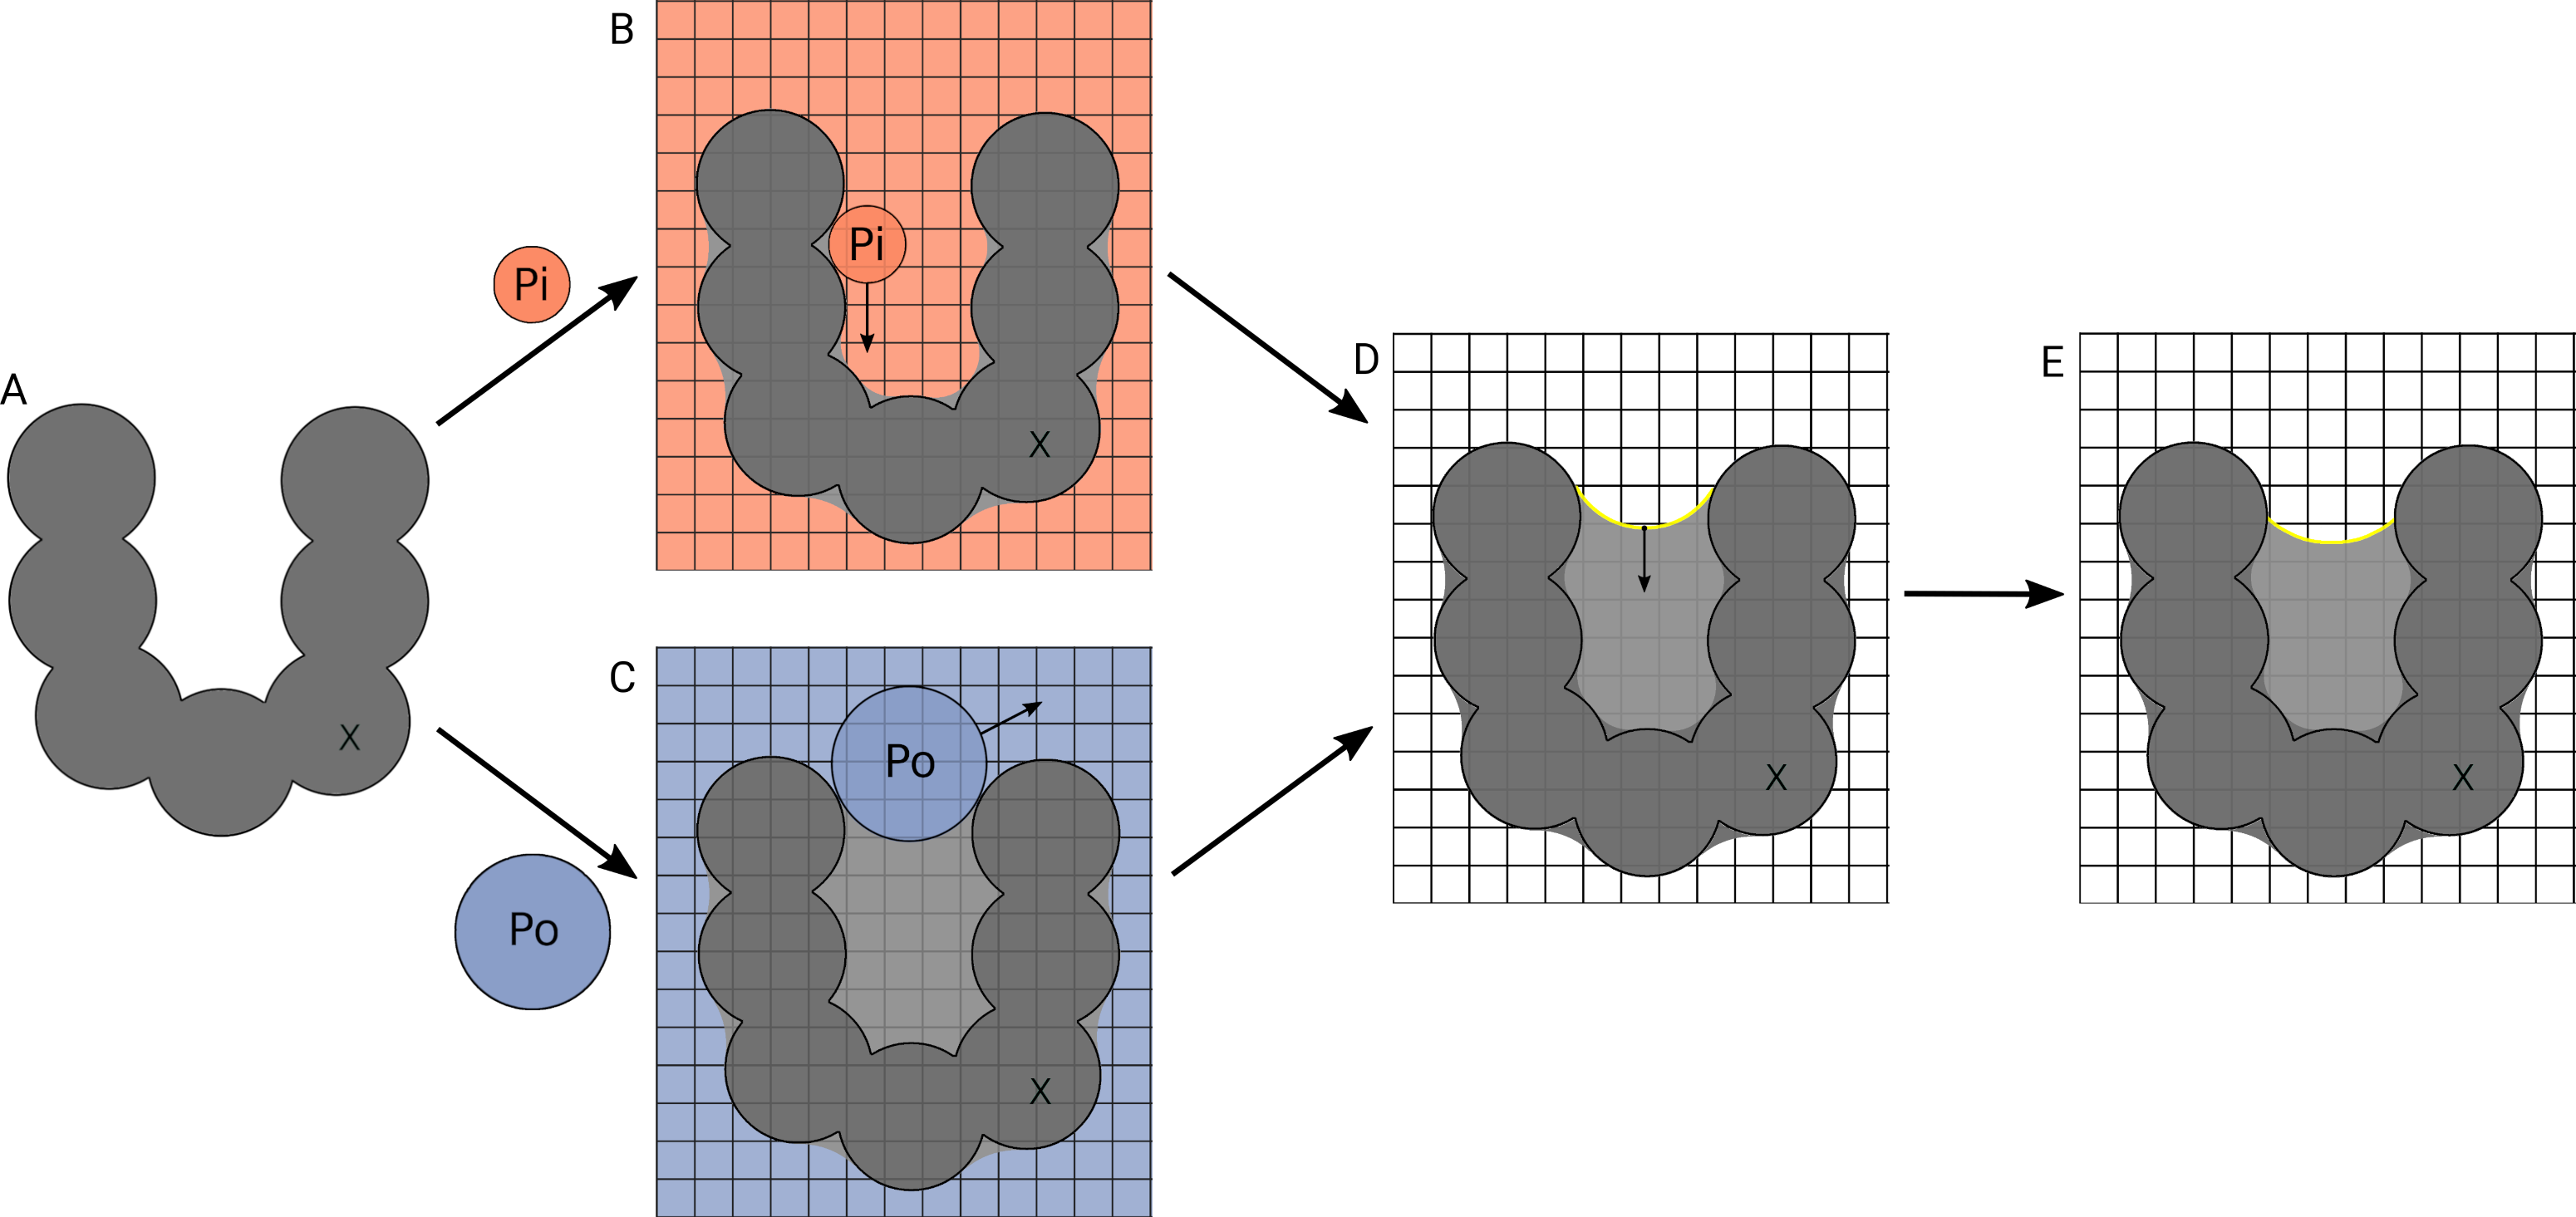
\includegraphics[scale=0.65]{images/kvfinder-suite-schema.png}}
  \centerline{\scriptsize{\textbf{Fonte:} Retirado de \cite{guerra2023B}.}}
  \caption[Representação esquemática do algoritmo de detecção de cavidades no KVFinder suite]{\textbf{Representação esquemática do algoritmo de detecção de cavidades no KVFinder suite.} \textbf{(A)} Uma estrutura biomolecular X, composta por átomos modelados como esferas rígidas com raios de van der Waals, é inserida em uma grade 3D. \textbf{(B)} A sonda \textit{Probe In} (Pi) percorre a superfície da estrutura, movendo-se pelos pontos da grade (laranja). \textbf{(C)} Em seguida, a sonda \textit{Probe Out} (Po) percorre os pontos acessíveis em azul. \textbf{(D)} Os pontos de cavidade (cinza claro) são definidos como a diferença entre os pontos acessíveis das sondas. Os pontos não alcançados por Pi (cinza escuro) definem a SES (padrão) ou a SAS, dependendo da representação de superfície escolhida pelo usuário. \textbf{(E)} Por fim, é aplicado um procedimento de remoção por distância para eliminar os pontos de cavidade que estão próximos à fronteira da cavidade-solvente (linha amarela).}
  \label{fig:kvfinder-suite-schema}
\end{figure}

É importante destacar que a ferramenta KVFinder \cite{oliveira2014}, originalmente publicada em 2014, está descontinuada. No entanto, novas implementações foram desenvolvidas para aprimorar o desempenho computacional e a usabilidade, resultando nas ferramentas parKVFinder \cite{guerra2020}, pyKVFinder \cite{guerra2021} e KVFinder-web \cite{guerra2023A}. Cada uma dessas ferramentas aborda diferentes demandas da comunidade científica de forma flexível. A caracterização das cavidades nessas ferramentas inclui descritores morfológicos, como volume, área, forma e profundidade, bem como descritores topológicos, como os resíduos de interface que cercam as cavidades, e descritores físico-químicos, como a hidrofobicidade. Para mais informações sobre o KVFinder suite, veja a Seção \ref{sec:kvfinder-suite}.

\subsubsection{Fpocket}

O Fpocket \cite{fpocket} é uma ferramenta baseada em tesselação que realiza a detecção de bolsões com base no conceito de \textalpha-esferas, introduzido por \cite{liang1998}. O algoritmo de detecção de cavidade (Figura \ref{fig:fpocket-schema}) determina o conjunto de \textalpha-esferas a partir da estrutura-alvo, utilizando o pacote \textit{qhull}, e elimina esferas fora de um tamanho de raio mínimo e máximo. As cavidades são agrupamentos de \textalpha-esferas, formadas com base em relações de proximidade e vizinhança, sendo que cavidades não interessantes são removidas da análise posterior. As cavidades restantes são avaliadas usando um conjunto de descritores dpocket \cite{fpocket} e classificadas de acordo com sua suposta capacidade de ligação a uma pequena molécula.

\begin{figure}[ht]
  \centerline{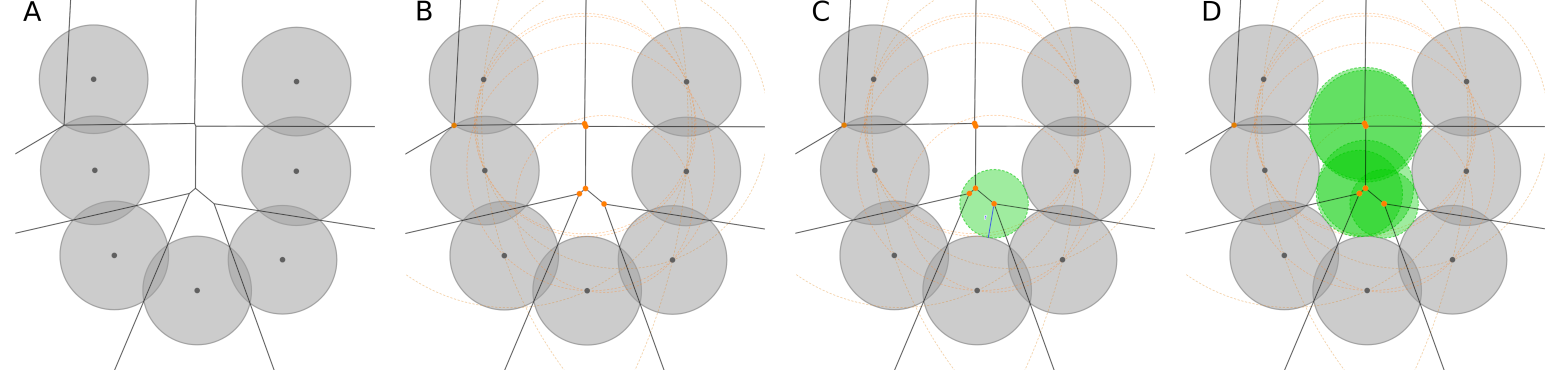
\includegraphics[scale=0.24]{images/fpocket-schema.png}}
  \centerline{\scriptsize{\textbf{Fonte:} Retirado de \cite{guerra2023B}.}}
  \caption[Representação esquemática do algoritmo de detecção de cavidades no Fpocket]{\textbf{Representação esquemática do algoritmo de detecção de cavidades no Fpocket.} \textbf{(A)} Diagrama de Voronoi dos centros atômicos. \textbf{(B)} Semelhante a uma esfera de Voronoi (círculos laranja pontilhados). \textbf{(C)} Exemplo de uma \textalpha-esfera (região verde); ela é centrada em um vértice de Voronoi (pontos laranja) e cresce até se tornar tangente aos átomos da superfície. \textbf{(D)} Cluster de \textalpha-esferas que preenchem o sítio de ligação.}
  \label{fig:fpocket-schema}
\end{figure}

\subsubsection{GHECOM}

O GHECOM (\textit{Grid-based HECOMi finder}) \cite{ghecom} é uma ferramenta baseada em grade e esfera que detecta bolsos profundos e rasos, utilizando várias sondas esféricas diferentes (Figura \ref{fig:ghecom-schema}). O algoritmo de detecção de cavidade combina operações básicas de erosão e dilatação, da morfologia matemática, com diferentes sondas esféricas para relatar a abertura-fechamento de uma forma molecular-alvo, revelando assim bolsos profundos e rasos (\textit{multi-scale pockets}, em inglês). Dessa forma, um método de agrupamento de ligação simples agrupa regiões de bolsos e posteriormente estima seus volumes. Além disso, o GHECOM relaciona o volume e a profundidade de pontos por resíduo ou átomo em uma métrica chamada \textit{pocketness}, que indica o quanto eles contribuem para a interação com ligantes.

\begin{figure}[ht]
  \centerline{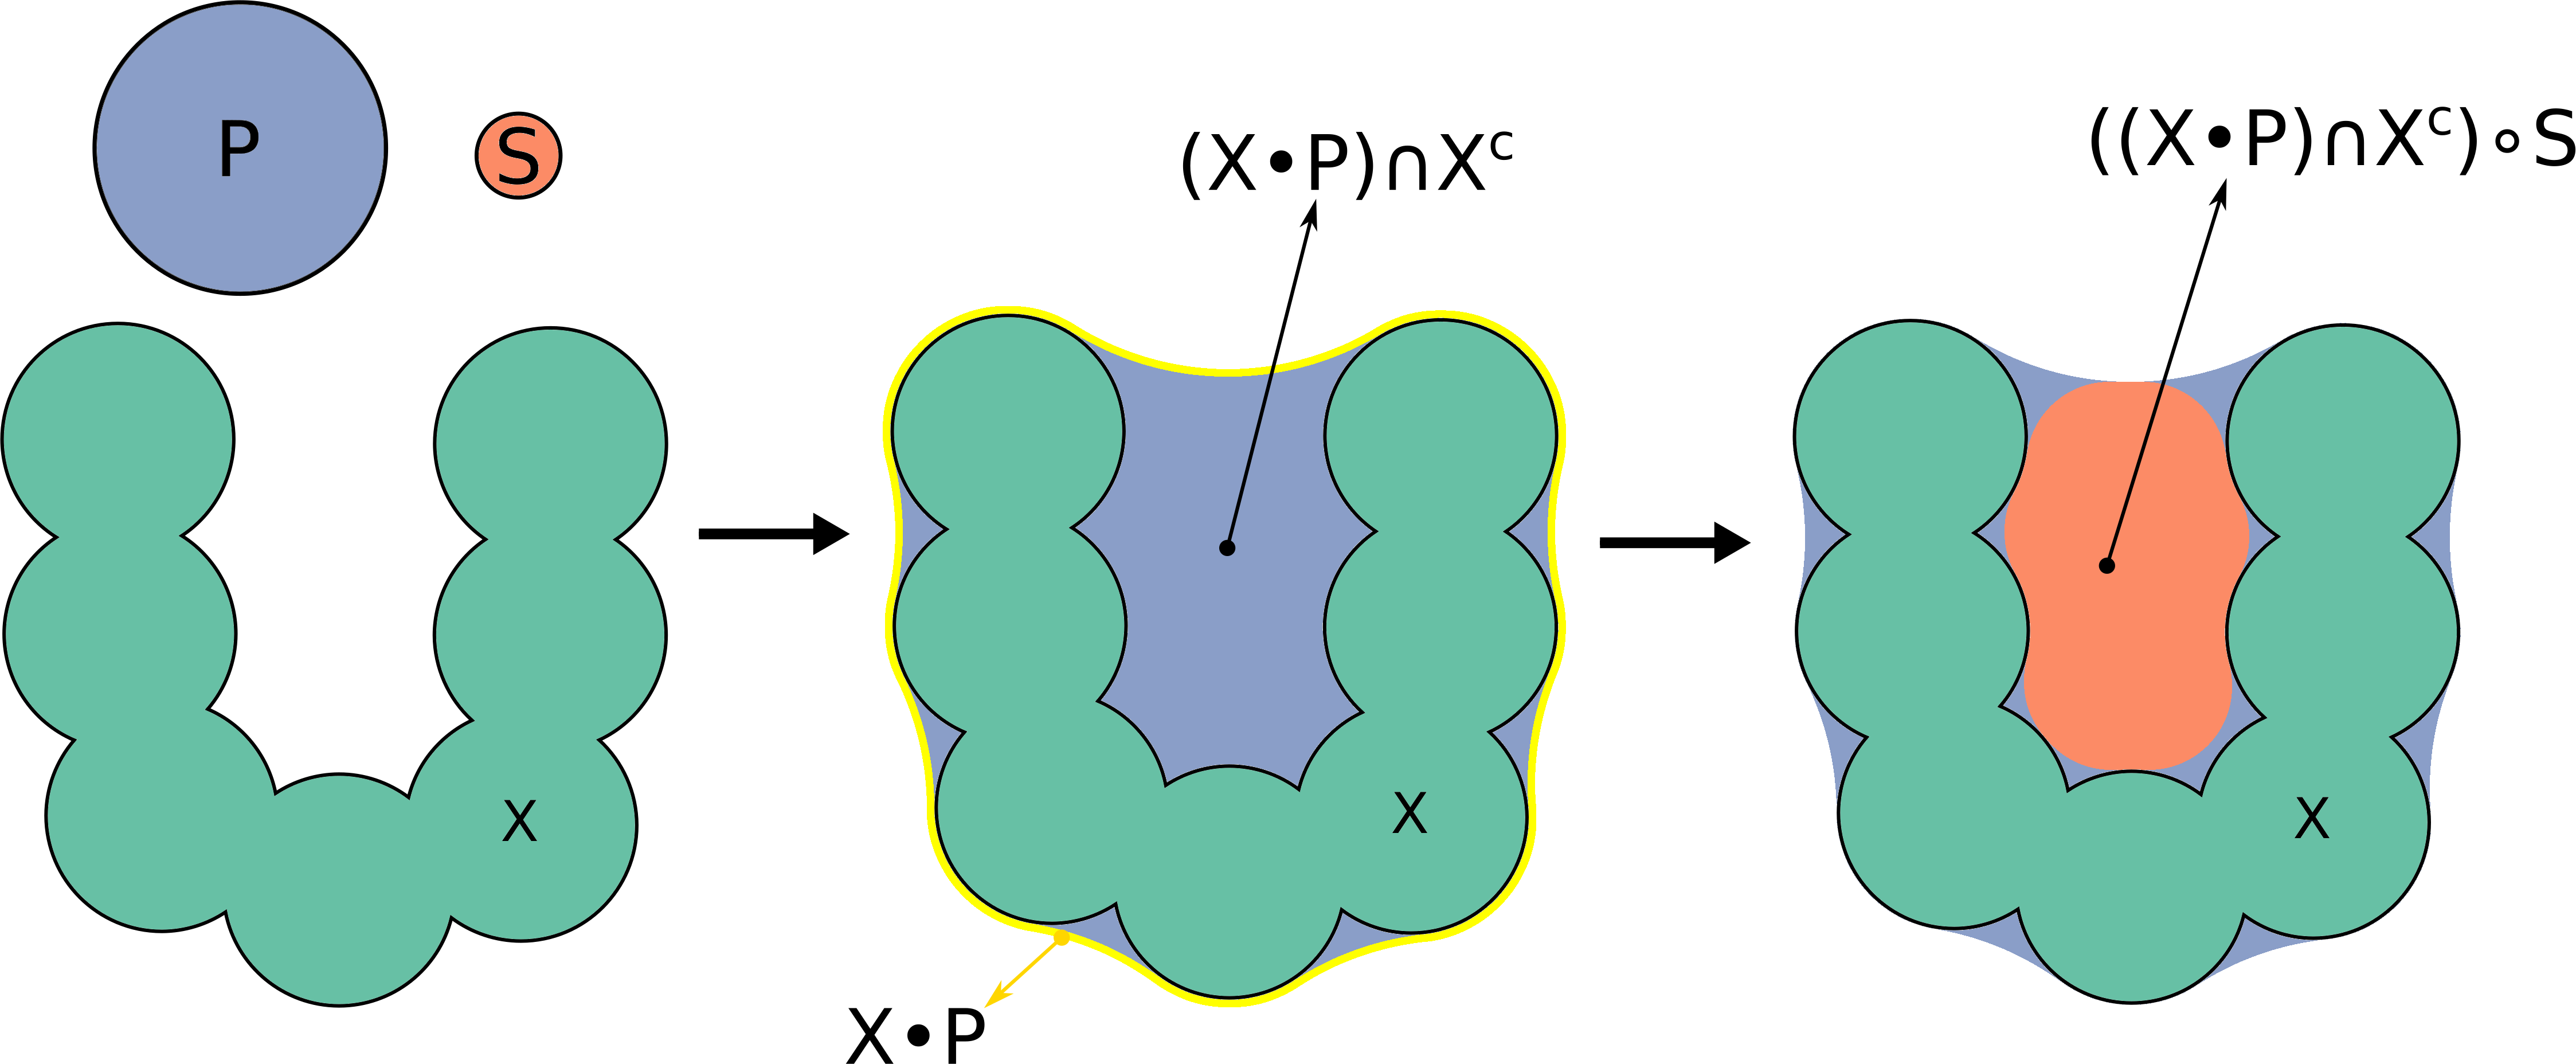
\includegraphics[scale=0.6]{images/ghecom-schema.png}}
  \centerline{\scriptsize{\textbf{Fonte:} Retirado de \cite{guerra2023B}.}}
  \caption[Representação esquemática do algoritmo de detecção de bolsões no GHECOM]{\textbf{Representação esquemática do algoritmo de detecção de bolsões no GHECOM.} Uma estrutura biomolecular (região verde; $X$) é fechada por uma sonda esférica P (esfera azul), definindo a região delimitada pelo contorno amarelo. Em seguida, a interseção de X fechado por P ($X \bullet P$) e o espaço fora da proteína ($X^c$) define a região não acessível à sonda P (região azul; $(X \bullet P) \cap X^c$). Posteriormente, essa região é aberta por uma sonda esférica S (esfera laranja), onde P é maior que S. Por fim, o bolsão (região laranja; $((X \bullet P) \cap X^c) \circ S$) é definido pelo espaço fora da forma molecular não acessível a P, mas acessível a S. Para detecção em múltiplas escalas, são usados diferentes tamanhos da sonda esférica P.}
  \label{fig:ghecom-schema}
\end{figure}

\subsubsection{CAVER}

O CAVER \cite{caver} foi originalmente uma ferramenta baseado em grade e superfície para o cálculo de túneis e canais, que posteriormente foi aprimorado no CAVER 3.0 \cite{caver3}, substituindo a grade alinhada aos eixos por uma abordagem de diagrama de Voronoi. A interface gráfica do usuário, CAVER Analyst 2.0 \cite{caveranalyst2}, incorpora o CAVER 3.0, que auxilia visualmente os usuários nos cálculos de túneis e cavidades. O algoritmo de detecção de cavidades (Figura \ref{fig:caver-schema}) constrói um pseudo-diagrama de Voronoi de uma estrutura biomolecular alvo. A partir dele, o CAVER 3.0 identifica caminhos como grafos compostos por vértices e arestas de Voronoi. Esses caminhos se assemelham a túneis que conectam cavidades ao solvente circundante e são caracterizados por comprimento, raio médio e raio da garganta. Além disso, CAVER Analyst 2.0 também identifica regiões de espaço vazio, onde uma sonda pequena pode entrar de fora, mas uma sonda grande não pode, aplicando uma abordagem similar às descritas no KVFinder suite (Figura \ref{fig:kvfinder-suite-schema}) e GHECOM (Figura \ref{fig:ghecom-schema}).

\begin{figure}[ht]
  \centerline{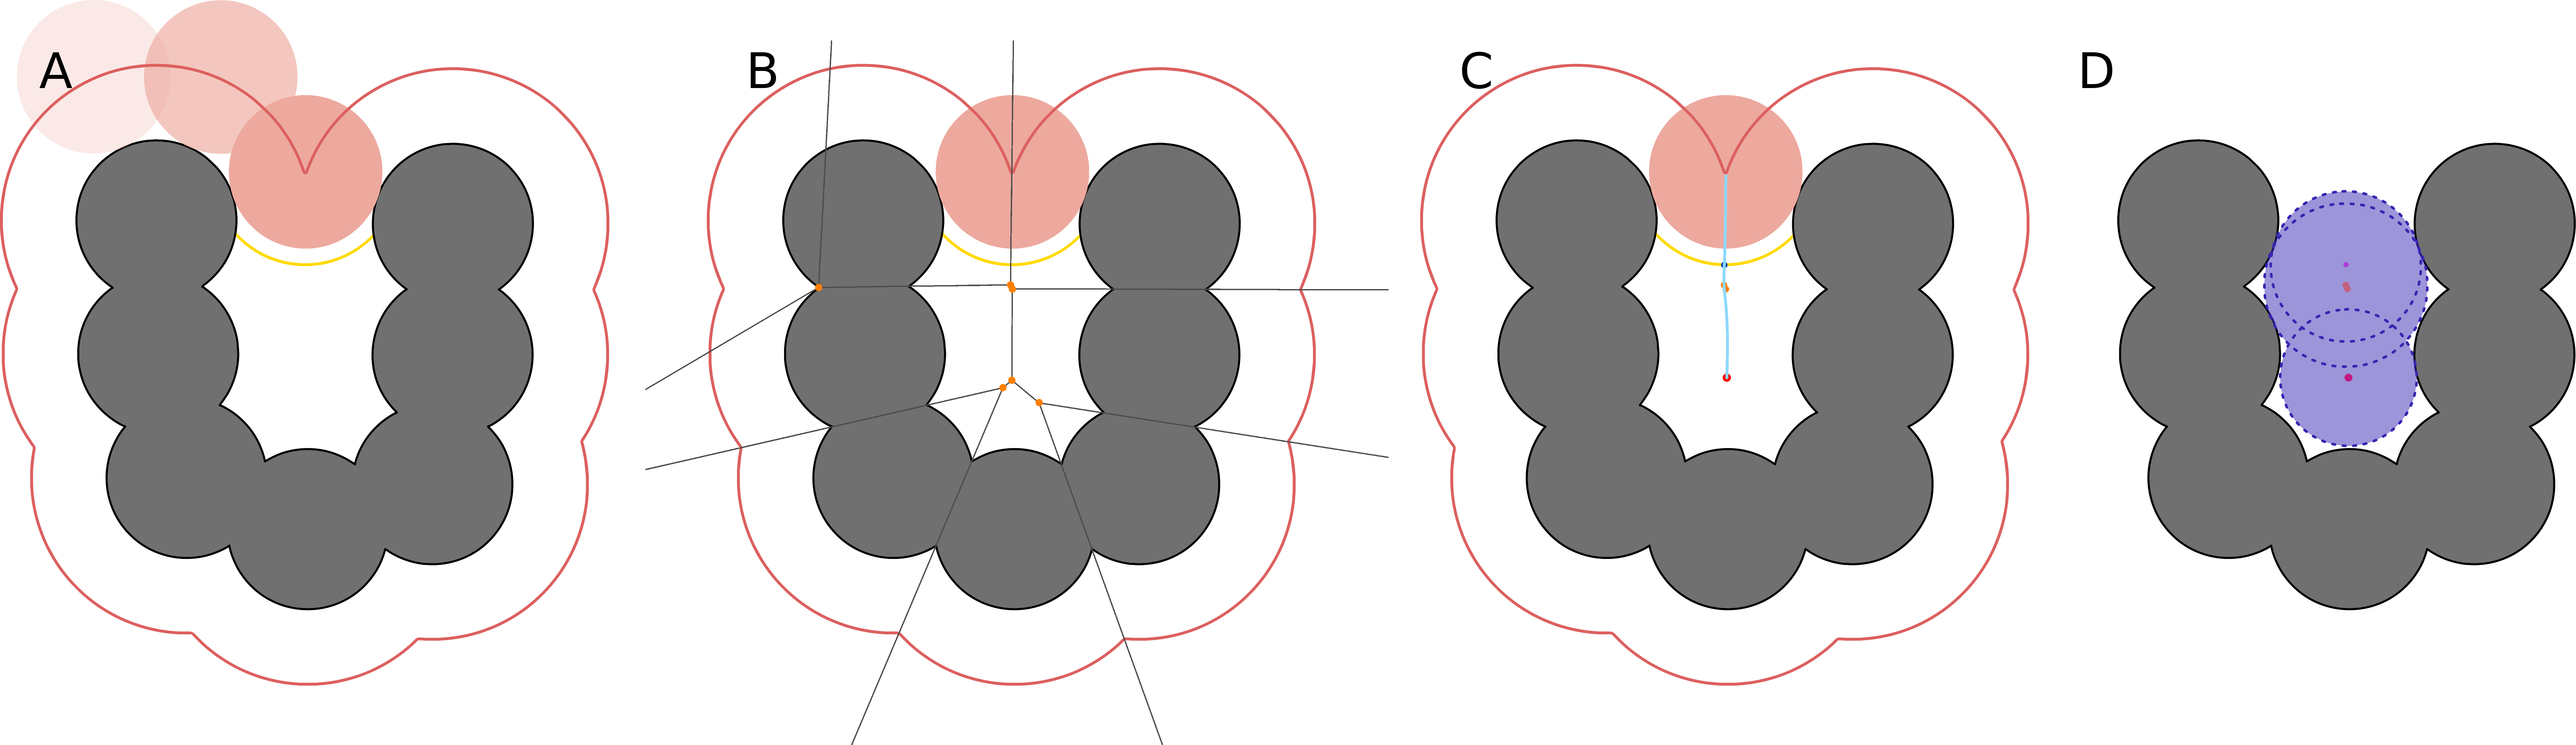
\includegraphics[scale=0.18]{images/caver-schema.png}}
  \centerline{\scriptsize{\textbf{Fonte:} Retirado de \cite{guerra2023B}.}}
  \caption[Representação esquemática do algoritmo de detecção de canais e túneis no CAVER 3.0 e CAVER Analyst 2.0]{\textbf{Representação esquemática do algoritmo de detecção de canais e túneis no CAVER 3.0 e CAVER Analyst 2.0.} \textbf{(A)} Uma forma molecular é inspecionada por uma sonda esférica, chamada \textit{shell probe}, com um raio especificado pelo parâmetro \textit{shell radius}, para definir uma superfície externa SAS (linha vermelha). A partir dela, uma distância especificada pelo parâmetro \textit{shell depth} é removida para definir uma superfície interna (linha amarela). \textbf{(B)} Um pseudo-diagrama de Voronoi é construído com base na forma molecular. Vértices de Voronoi (pontos laranja) são usados para criar as linhas centrais do túnel/canal. \textbf{(C)} Um ponto de partida (ponto vermelho) é um parâmetro definido pelo usuário, definido como o centro de massa da forma molecular, e um ponto final (ponto azul) é definido no centro da superfície interna. A partir do ponto de partida, a linha central passa por arestas e vértices de Voronoi para formar um túnel/canal até a superfície externa e passa pelo ponto final. \textbf{(D)} Esferas são ajustadas em todos os pontos da linha central, do ponto de partida ao ponto final, o que define o raio do gargalo (abertura) ao longo do túnel e/ou canal.}
  \label{fig:caver-schema}
\end{figure}

% Cavity characterization 

% Maybe describe importance of cavity characterization to identify functionally relevant cavities

%%% Chapter 2

\chapter{Objetivos}

\section{Objetivo geral}

Este trabalho tem como objetivo o desenvolvimento de uma plataforma computacional, denominada \textbf{KVFinder suite}, para estudo de sistemas biomoleculares em biologia estrutural.

\section{Objetivos específicos}

Os objetivos específicos incluem: 

\begin{itemize}
  \item Aprimoramento e desenvolvimento de descritores de propriedades do KVFinder suite;
  \item Implementação de diferentes codificações para biomoléculas e sítios de ligação; % cavidade, resíduos e grafos
  \item Desenvolvimento de ferramenta para ciência de dados e protocolos automatizados; % pyKVFinder
  \item Desenvolvimento de um serviço \textit{web} para análise de sítios de ligação; % KVFinder-web
  \item Desenvolvimento de ferramenta para análises dinâmica molecular; % KVFinderMD
  \item Desenvolvimento de um programa para representação gráfica de regiões expostas de biomoléculas. % SERD
\end{itemize}

%%% Chapter 3

\chapter{Codificação de biomoléculas e sítios de ligação}

% \begin{itemize}
%   \item Explique as diferentes representações de biomoléculas que podem ser usadas em simulações computacionais e em estudos de sítios de ligação;
%   \item Descreva em detalhes as representações usadas no KVFinder suite, como modelos de pontos, modelos de esferas, superfícies moleculares e mapas de densidade eletrônica;
%   \item Explique como cada uma dessas representações pode ser usada para identificar sítios de ligação em biomoléculas.
%  \end{itemize}

A codificação de biomoléculas e sítios de ligação desempenha papel fundamental na biologia estrutural, permitindo a representação e análise computacional de informações biológicas complexas. Esse processo converte informações biológicas em formatos compreensíveis e adequados para processamento por algoritmos e programas em sistemas computacionais. A codificação envolve a atribuição de valores ou categorias aos componentes biológicos, \eg, átomos, aminoácidos e bases nitrogenadas, para descrever ocupância, localização, forças, características físico-químicas e/ou propriedades estruturais. 

Na biologia estrutural, a codificação de dados é importante para realizar análises avançadas, \eg modelagem molecular, simulações de dinâmica molecular e predição de interações. Existem várias aplicações que exemplificam a codificação de dados biológicas para análises computacionais. Por exemplo, na modelagem molecular, uma proteína pode ser codificada usando códigos de uma letra para representar os diferentes aminoácidos, como ocorre na representação de sequência de proteínas, para predizer o dobramento de proteínas, como aplicado no ESMFold \cite{lin2022}. Na simulação de dinâmica molecular, as coordenadas 3D de átomos ou conjunto de átomos, juntamente com vetores que representam forças ou outros atributos, são utilizados para representar a estrutura de uma biomolécula, como no GROMACS \cite{gromacs} ou AMBER \cite{amber} em simulações em escala atomística (\textit{fine-grained molecular dynamics simulation}) e no CafeMol em simulações em escala grosseiras (\textit{coarse-grained molecular dynamics simulation}) \cite{kenzaki2011}. Além disso, os sítios de ligação, após identificados por algoritmos computacionais, são codificados de diferentes maneiras para análises posteriores. Os sítios de ligação podem codificados para representar as características físico-químicas e estruturais de uma região de uma biomolécula, como as grades 3D utilizadas no KVFinder suite \cite{oliveira2014,guerra2020,guerra2021,guerra2023B}, ou as coordenadas 3D dos átomos, como no fpocket \cite{fpocket}.

Ao trabalhar com modelos computacionais para o estudo de biomoléculas, a codificação é essencial para a abstração e representação dos dados biológicos de forma computacional. Essa abstração é crucial para o desenvolvimento de ferramentas computacionais voltadas ao estudo de sistemas biomoleculares. Aqui, apresentamos as codificações implementadas para biomoléculas e sítios de ligação, \ie, representação em grade 3D, representação topológica e representação gráfica.

\section{Representação em grade tridimensional}

As biomoléculas e seus sítios de ligação podem ser representadas em uma grade 3D subdividida em voxels (\textit{volumetric pixel}, em inglês). A grade 3D é uma estrutura de dados que armazena valores em uma matriz tridimensional, onde cada elemento da matriz é denominado voxel. O voxel representa um ponto discreto de dados em uma grade regular no espaço tridimensional, sendo que cada ponto pode conter mais de uma informação a fim de representar diferentes propriedades em uma certa porção de espaço de maneira simples e efetiva (Figura \ref{fig:voxel}). Em computação, a grade 3D é uma estrutura de dados comumente utilizada em aplicações de processamento de imagens e visão computacional, como em reconstrução de imagens, segmentação de imagens e detecção de objetos. 

\begin{figure}[ht]
  \centerline{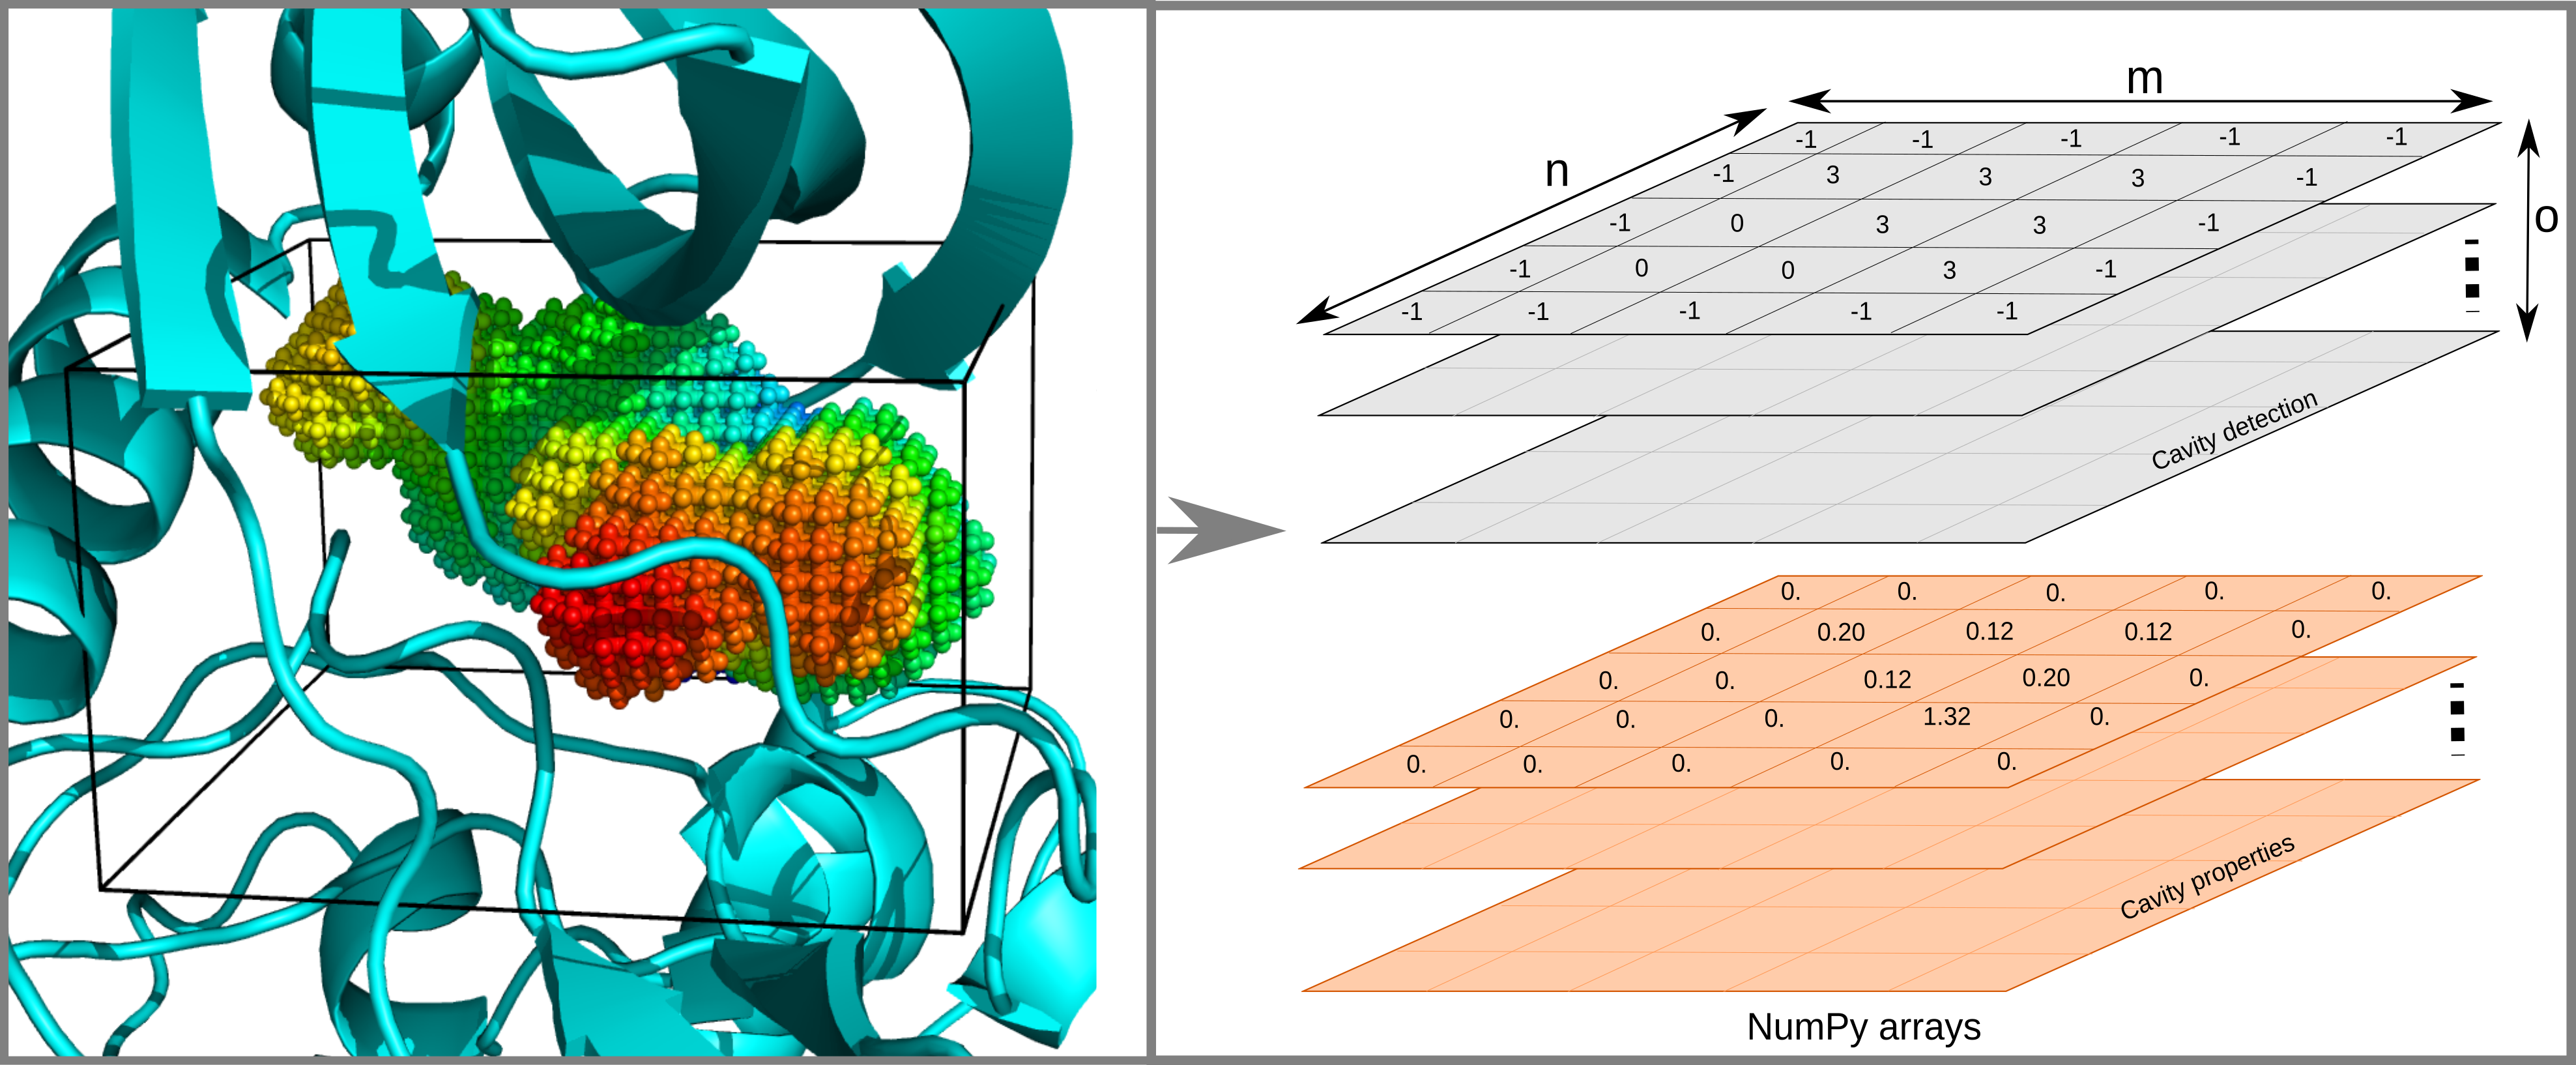
\includegraphics[scale=0.75]{images/voxels.png}}
  \centerline{\scriptsize{\textbf{Fonte:} Retirado de \cite{guerra2021}.}}
  \caption[Representação esquemática de biomoléculas e seus sítios de ligação representadas em grade tridimensional]{\textbf{Representação esquemática de biomoléculas e seus sítios de ligação representadas em grade tridimensional.} Com base em uma grade tridimensional com dimensões (m, n, o), cada elemento corresponde a uma região de cavidade (>1), espaço vazio (1), biomolécula (0) ou solvente (-1). Além disso, propriedades também são armazenadas na mesma estrutura de dados, correspondendo ao valor da propriedade na região.}
  \label{fig:voxel}
\end{figure}

Dentre as diversas representações de superfície molecular, a grade tridimensional composta por voxels é a mais simples e apropriada para a representação de múltiplas propriedades em várias condições, pois cada voxel da grade tridimensional pode acumular diferentes informações. Além disso, a grade 3D é uma estrutura de dados eficiente para armazenar e acessar valores e/ou atributos em uma posição 3D, permitindo a realização de operações matemáticas e lógicas em uma região 3D. 

% Essa representação é útil para identificar regiões de interesse em biomoléculas, como sítios de ligação, e para realizar análises de propriedades físico-químicas e estruturais, como a distribuição de cargas e a distribuição de propriedades hidrofóbicas. 

\subsection{Representação de superfícies moleculares}

A representação de superfícies moleculares é uma etapa fundamental na modelagem e análise de biomoléculas. Nessa abordagem, as biomoléculas são descritas por meio de um modelo de esfera rígida, que considera as posições e raios atômicos para representar a superfície molecular. Existem três formulações matemáticas comumente utilizadas para representar as superfícies moleculares (Figura \ref{fig:surface-representation}):

\begin{enumerate}[label=\textbf{(\Alph*)}]
  \item \textbf{superfície de vdW:} representa cada átomo por uma esfera cujo raio é proporcional ao seu raio de van der Waals. A superfície de vdW é representada como a união desses átomos esféricos; 
  \item \textbf{SAS:} representa as regiões de uma molécula que podem ser acessadas por uma molécula de solvente (\eg, uma molécula de água), que é aproximada por uma sonda esférica;
  \item \textbf{SES:} é semelhante ao SAS, mas considera-se a casca externa da sonda, em vez do centro da sonda.
\end{enumerate}

\begin{figure}[ht]
  \centerline{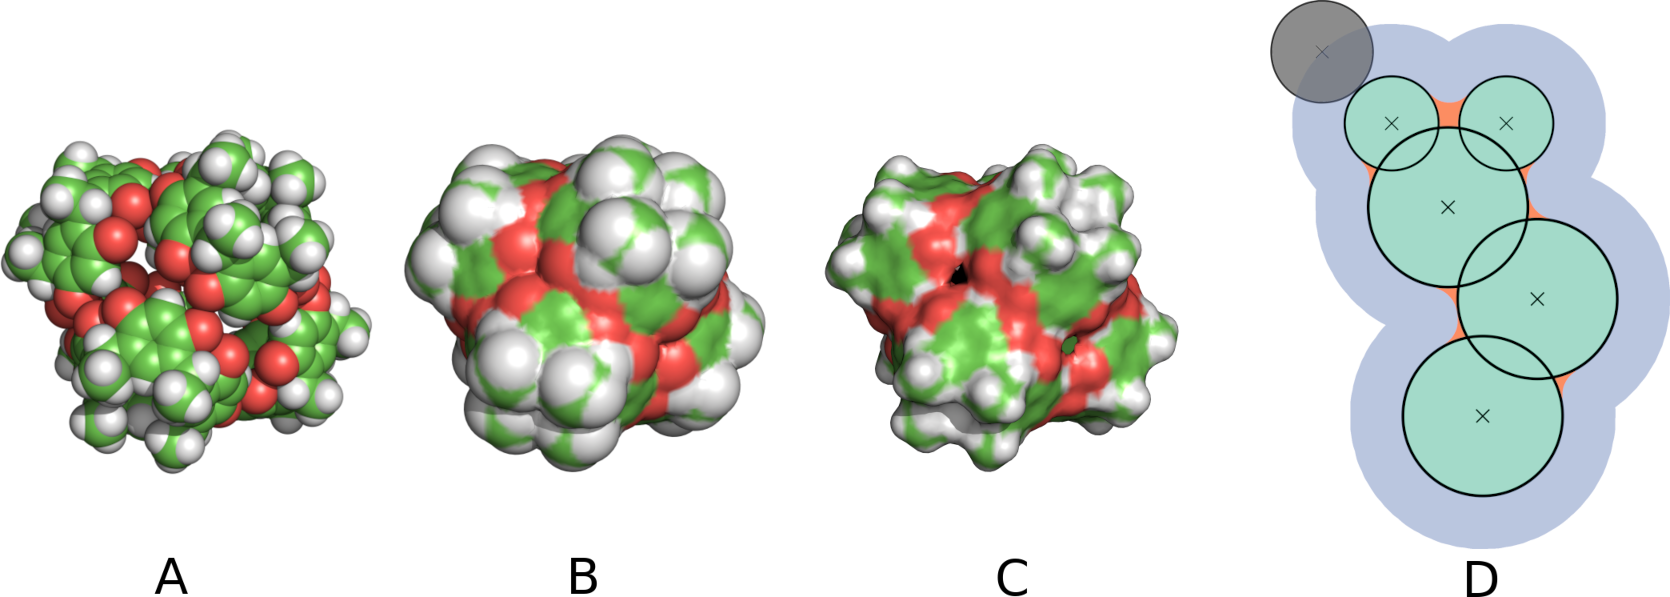
\includegraphics[scale=0.8]{images/surface-representation.png}}
  \centerline{\scriptsize{\textbf{Fonte:} Retirado de \cite{guerra2023B}.}}
  \caption[Representações de superfície molecular]{\textbf{Representações de superfície molecular.} \textbf{(A)} Superfície de vdW. \textbf{(B)} SAS. \textbf{(C)} SES. Imagens geradas com PyMOL para a gaiola supramolecular (resorcin[4]areno-hexamérica). \textbf{(D)} Representação esquemática 2D das superfícies moleculares. A superfície de vdW (verde) é composta por átomos representados como esferas verdes. Uma sonda esférica (cinza), representando uma molécula de solvente, rola sobre os átomos da molécula para definir SES e SAS. O SES é definido pela superfície de vdW (verde) e pelo espaço não alcançado pela sonda esférica (laranja). O SAS é definido pelo envelope alcançado pelo centro da sonda esférica (azul).}
  \label{fig:surface-representation}
\end{figure}

\section{Representação pela topologia}

Em vez de representar os dados estruturais por meio de voxels em uma grade 3D, as biomoléculas e seus sítios de ligação também podem ser representados pela topologia (Figura \ref{fig:topology}), seguindo abordagens semelhantes às simulações de dinâmica molecular, como GROMACS \cite{gromacs}, AMBER \cite{amber} e CafeMol \cite{kenzaki2011}. Nessa representação, átomos, resíduos e/ou bases nucleotídicas são modelados como esferas rígidas (modelos de esfera dura) com coordenadas tridimensionais (x, y, z), juntamente com vetores (\eg, forças, velocidades e acelerações) e propriedades (\eg, massa, carga e raio de van der Waals).

% Figura de representação topológica.

Porém, ao estudarmos regiões de interação, é necessário filtrar as áreas de interesse, como sítios de ligação ou superfície exposta ao solvente, para realizar análises estruturais e funcionais específicas. Essa representação topológica permite uma análise mais focada e detalhada das interações e características estruturais que são importantes para a função biológica. Além disso, essas informações topológicas podem ser utilizadas em estudos de docking molecular, design de fármacos e predição de interações moleculares, contribuindo para o desenvolvimento de novos compostos terapêuticos.

\section{Representação em grafos}

% A representação das IPLs em grafos é menos complexa do que as estruturas atomísticas e podem mostrar com mais clareza os diferentes tipos de interação entre os resíduos, além de permitir a inclusão de atributos nos elementos do grafo. Esse tipo de representação já foi utilizado na detecção de sítios ativos e resíduos estruturalmente relevantes de proteínas, na predição de sua estrutura e na identificação e caracterização de cavidades em dinâmicas moleculares (VISHVESHWARA et al., 2002; LINDOW et al., 2013).

% Um grafo é definido como um par contendo um conjunto de vértices representando os nós e um conjunto de arestas que conectam esses nós. Essas arestas podem estar associadas a um atributo que denota alguma característica dessa conexão (MASON; VERWOERD, 2007). 
% Os grafos podem ser divididos em duas classes: direcionados e não-direcionados. Grafos direcionados contém arestas com um nó inicial e um terminal, enquanto que as arestas de grafos não-direcionados não possuem ordenação. Grafos não-direcionados têm sido bastante usados como modelos para redes de interação proteína-proteína, onde cada aresta representa uma interação. (PAVLOPOULOS et al., 2011; LINDOW et al., 2013).

% Os grafos possuem propriedades que podem ser calculadas a partir dos vértices e arestas. Uma dessas propriedades é o “caminho”, que é definido como uma sequência de vértices sem arestas repetidas, de modo que a distância entre dois vértices é o número de arestas referente ao caminho mais curto entre eles. A partir dessa medida pode ser calculado o diâmetro de um grafo, definido pela máxima distância encontrada dentre todos os pares possíveis de vértices (MASON; VERWOERD, 2007).

% Além disso, o conceito de centralidade pode ser empregado para determinação dos nós mais importantes de um grafo. Quatro tipos de centralidades são normalmente utilizados: 1) centralidade de grau, que mede o número de conexões que um vértice possui com os demais; 2) centralidade de proximidade, relacionada às distâncias de um determinado vértice em relação aos demais; 3) centralidade de intermediação, que calcula a frequência de um determinado vértice nas distâncias entre os pares de nós; 4) centralidade autovetor, que mede a importância de um nós com base na sua vizinhança. Em estudos com redes de interação gênicas e de proteínas, vértices com maior valor de centralidade de grau representaram genes e proteínas essenciais ao organismo de estudo. Ademais, cálculos de centralidades de proximidade já foram utilizados em análises de redes metabólicas e para predição, em proteínas, de sítios de ligação a substratos, íons, co-fatores e sítios alostéricos (MASON; VERWOERD, 2007; AMITAI et al., 2004).

%%% Chapter 4

\chapter{Plataforma KVFinder suite \label{sec:kvfinder-suite}}

% https://cnpemcamp-my.sharepoint.com/:w:/r/personal/joao_guerra_lnbio_cnpem_br/_layouts/15/Doc.aspx?sourcedoc=%7BD0C80180-AF7E-412F-B94E-6C38D8D4C946%7D&file=Relat%C3%B3rio%20Plataforma%20Biologia%20Computacional%202022.2.docx&action=default&mobileredirect=true

% \begin{itemize}
%   \item Descreva cada um dos programas do KVFinder suite, explicando seus objetivos e principais características;
%   \item Apresente exemplos de aplicação de cada programa em estudos de sítios de ligação em biomoléculas, mostrando os resultados obtidos e como eles contribuíram para a compreensão da função biológica das moléculas estudadas;
%   \item Explique como os resultados obtidos pelo KVFinder suite podem ser validados experimentalmente.
%  \end{itemize}

% Composto por cinco ferramentas principais, o KVFinder Suite oferece uma ampla gama de funcionalidades para auxiliar na análise estrutural e no estudo de interações biomoleculares. A seguir, descrevemos cada uma das ferramentas e suas principais características.

Processos biológicos são modulados por interações entre biomoléculas, variando de pequenas moléculas, como íons, até macromoléculas, como proteínas e ácidos nucleicos. Para o processo de interação, ligantes geralmente interagem em sítios de ligação específicos formados por fendas expostas ao solvente ou cavidades enterradas nos receptores. As interações receptor-ligante, como interações proteína-proteína (IPP) e proteína-ligante (IPL), são consequência da complementariedade espacial, estrutural e físico-química, que governam o reconhecimento molecular entre o par de interação, restringindo assim a um pequeno número de ligantes a interação eficiente com um dado receptor alvo. A identificação e avaliação de cavidades permite o entendimento da estrutura terciária da biomolécula e também de seus supostos sítios de ligação ao ligante, desempenhando um papel estratégico no desenvolvimento de novos fármacos. Neste cenário, o Laboratório de Biologia Computacional (LBC) integrou ferramentas de detecção e caracterização de sítios de ligação de biomoléculas em uma plataforma, chamada KVFinder-suite, contemplando os programas publicados anteriormente, parKVFinder (https://github.com/LBC-LNBio/parKVFinder) [1] e pyKVFinder (https://github.com/LBC-LNBio/pyKVFinder) [2]. Concomitantemente, o grupo está desenvolvendo novas ferramentas, como o KVFinder-web, SERD e KVFinderMD para integrarem a plataforma. 

\section{parKVFinder}

\section{pyKVFinder}

\subsection{Estimativa do volume molecular}

\cite{guerra2023B}

\section{KVFinder-web}

% Several web services have been proposed for the detection and/or characterization of binding sites in biomolecules. Amongst them, we could cite FpocketWeb (5), GHECOM (6), CaverWeb (7), CASTp (8), ConCavity (9), Depth (10), MoloVol (11) and 3DLigandSite (12).

O KVFinder-web é uma aplicação web de código aberto para detecção e caracterização de cavidades em qualquer tipo de estrutura biomolecular, que consiste em dois componentes independentes: um serviço web RESTful (KVFinder-web service) e uma interface web gráfica (KVFinder-web interface).  

O serviço web do KVFinder (KVFinder-web service) detecta e caracteriza espacialmente cavidades usando o parKVFinder, que implementa um método geométrico baseado em grade e esfera, para detectar cavidades em estruturas biomoleculares, com um sistema de dupla sonda [1, 2, 3]. O serviço web possui uma arquitetura Web-Fila-Trabalho (em inglês, Web-Queue-Worker), que processa as solicitações e respostas HTTP da interface web, gerencia os trabalhos e executa o parKVFinder nos trabalhos aceitos. O KVFinder-web service foi testado em um conjunto de dados de 1.000 domínios de proteínas únicos [1] com 6 conjuntos diferentes de parâmetros de detecção, mostrando consistência neste teste de alta demanda. 

A interface web do KVFinder (KVFinder-web interface; Figura 11), desenvolvida em R Shiny, disponibiliza as principais funcionalidades do KVFinder-web service, no qual os usuários podem carregar uma biomolécula alvo de um arquivo PDB ou pelo código PDB, personalizar parâmetros de detecção de cavidades e modos de execução, e baixar e visualizar resultados. A interface fornece uma maneira fácil e interativa de obter e visualizar os resultados da detecção de cavidades (Figura 12). Os volumes e áreas de cada cavidade são mostrados em uma tabela interativa, disponível para download no formato TOML. Um visualizador de biomoléculas, alimentado pelo motor NGL para R, exibe a estrutura biomolecular com suas cavidades, para download no formato PDB, e permite várias personalizações, por exemplo, realçar cavidades e exibir resíduos de interface ao redor das cavidades. A KVFinder-web interface está disponível para testes à equipe do CNPEM desde agosto de 2022 para projetos internos. 

Por fim, a disponibilização do KVFinder-web pretende ampliar o uso desta robusta ferramenta de detecção de cavidades na comunidade científica. Isso facilitará o processo de detecção e caracterização de cavidades, mesmo para usuários menos experientes, com impacto direto no desenvolvimento racional de medicamentos e no entendimento das estruturas das biomoléculas. 

\section{KVFinderMD}

% The protein-ligand and protein-protein interactions rely on the intrinsic dynamics of the target receptor, in which the classical lock and key model fails, and more recent binding models, e.g., induced-fit and conformation selection, thrive. Thus, molecular dynamics simulations are a useful tool to understand the underlying mechanisms of molecular recognition and, ultimately, the biomolecular function. In this scenario, we recently developed pyKVFinder, a Python package for detecting and characterizing biomolecular cavities in data science. Using it as a building block, we developed a new tool, called KVFinder for Molecular Dynamics analysis (KVFinderMD), to explore binding site dynamics in biomolecular structures of interest. Since the intrinsic biomolecule dynamics may change the shape and properties of the binding site over time, KVFinderMD can identify and characterize cavities in respect to volume, area, depth, hydropathy and interface residues, which are relevant properties to describe the molecular recognition process.

Em algumas circunstâncias, para a formação do complexo receptor-ligante, estes receptores utilizam sítios de ligação que não são facilmente identificados na forma não-ligada. Estas interações biomoleculares dependem da dinâmica intrínseca do receptor, nas quais o modelo clássico chave-fechadura falha, e modelos de ligação mais recentes, por exemplo, encaixe induzido e seleção de conformação, prosperam. Assim, as simulações de dinâmica molecular são uma ferramenta útil para entender os mecanismos de reconhecimento molecular e, em última análise, a função biomolecular. Nesse cenário, o LBC está desenvolvendo o KVFinderMD, usando o pyKVFinder [2] como bloco de construção, para explorar a dinâmica de sítios de ligação em estruturas biomoleculares de interesse farmacológico. Uma vez que a dinâmica intrínseca da biomolécula pode alterar a forma e as propriedades do sítio de ligação ao longo do tempo, o KVFinderMD pode identificar e caracterizar cavidades em relação ao volume, área, profundidade, hidropatia e resíduos de interface, que são propriedades relevantes para descrever o processo de reconhecimento molecular (Figura 14A). Além disso, também implementamos um algoritmo baseado em grafos, que considera distâncias alfa-carbono, beta-carbono ou quaisquer átomos, para descrever topologicamente o sítio de ligação (Figura 14B).

Como provas de conceito, aplicamos o KVFinderMD em importantes alvos terapêuticos, como HIV-1 protease e ALDH1/2. Para HIV-1 protease, descrevemos com sucesso as alterações conformacionais que definem o sítio ativo, causadas principalmente pelos movimentos β-hairpins. Ainda, usando a representação gráfica de cavidades, exploramos algoritmos de agrupamento não supervisionados, como agrupamento hierárquico, com diferentes métricas de distância para agrupar com sucesso as cavidades ao longo da trajetória do receptor. No caso das ALDH1/2, exploramos as diferenças topológicas e volumétricas entre os sítios de ligação do substrato de ALDH1 e ALDH2, o que dita a preferência por aldeídos menores e maiores entre eles. Os resultados desse trabalho foram apresentados em detalhe no IV Congresso de Estudantes do CNPEM (IV CEC). 

\section{SERD}

O reconhecimento molecular depende diretamente da acessibilidade de um ligante ao sítios de ligação do seu respectivo receptor. Os resíduos expostos ao solvente de uma biomolécula alvo (receptor) compõe o conjunto de átomos acessíveis a possíveis ligantes. Nesse cenário, a identificação destes resíduos possibilita um estudo mais direcionado aos hotspots de interação de um receptor alvo, com aplicações principalmente no estudo de docking proteína-proteína. O programa SERD (https://github.com/jvsguerra/SERD) aproxima uma molécula de solvente a uma esfera, a qual escaneia a superfície do receptor alvo para identificar as regiões que são acessíveis a esta sonda esférica. Após a identificação destes resíduos, o programa os representa na forma de grafos pela biblioteca networkX (https://networkx.org/), formando arestas até uma distância limite entre carbonos-alfa, carbonos-beta ou quaisquer átomos do resíduo e opcionalmente incluir essas distâncias como atributos das arestas desses grafos (Figura 13). 

\section{\textit{Benchmarking} das ferramentas disponíveis}

%%% Chapter 5

\chapter{Conclusões}

\begin{itemize}
  \item Comece explicando a importância dos sítios de ligação em biomoléculas e como eles afetam a função biológica das moléculas;
  \item Apresente os métodos experimentais e computacionais disponíveis para identificar e caracterizar sítios de ligação;
  \item Descreva brevemente os programas computacionais mais utilizados na área e suas principais características;
  \item Finalize apresentando o objetivo e a estrutura do seu trabalho.
 \end{itemize}

% As referências:
\bibliographystyle{unsrt}
\bibliography{phdquali}


% Os anexos, se houver, vêm depois das referências:
\appendix
\chapter{Anexo 1}
\chapter{Anexo 2}

\end{document}

% Table template

% \begin{table}
% \caption[Shorter table caption]{Table caption caption caption caption
%   caption caption caption caption caption caption caption caption caption
%   caption caption caption caption caption caption caption caption caption
%   caption caption.}
% \label{t:label0}
% \begin{center}
% \begin{tabular}{|c|c|}
% \hline
% a & b \\\hline
% c & d \\\hline
% \end{tabular}
% \end{center}
% \end{table}

% Figure template

% \begin{figure}
% \centerline{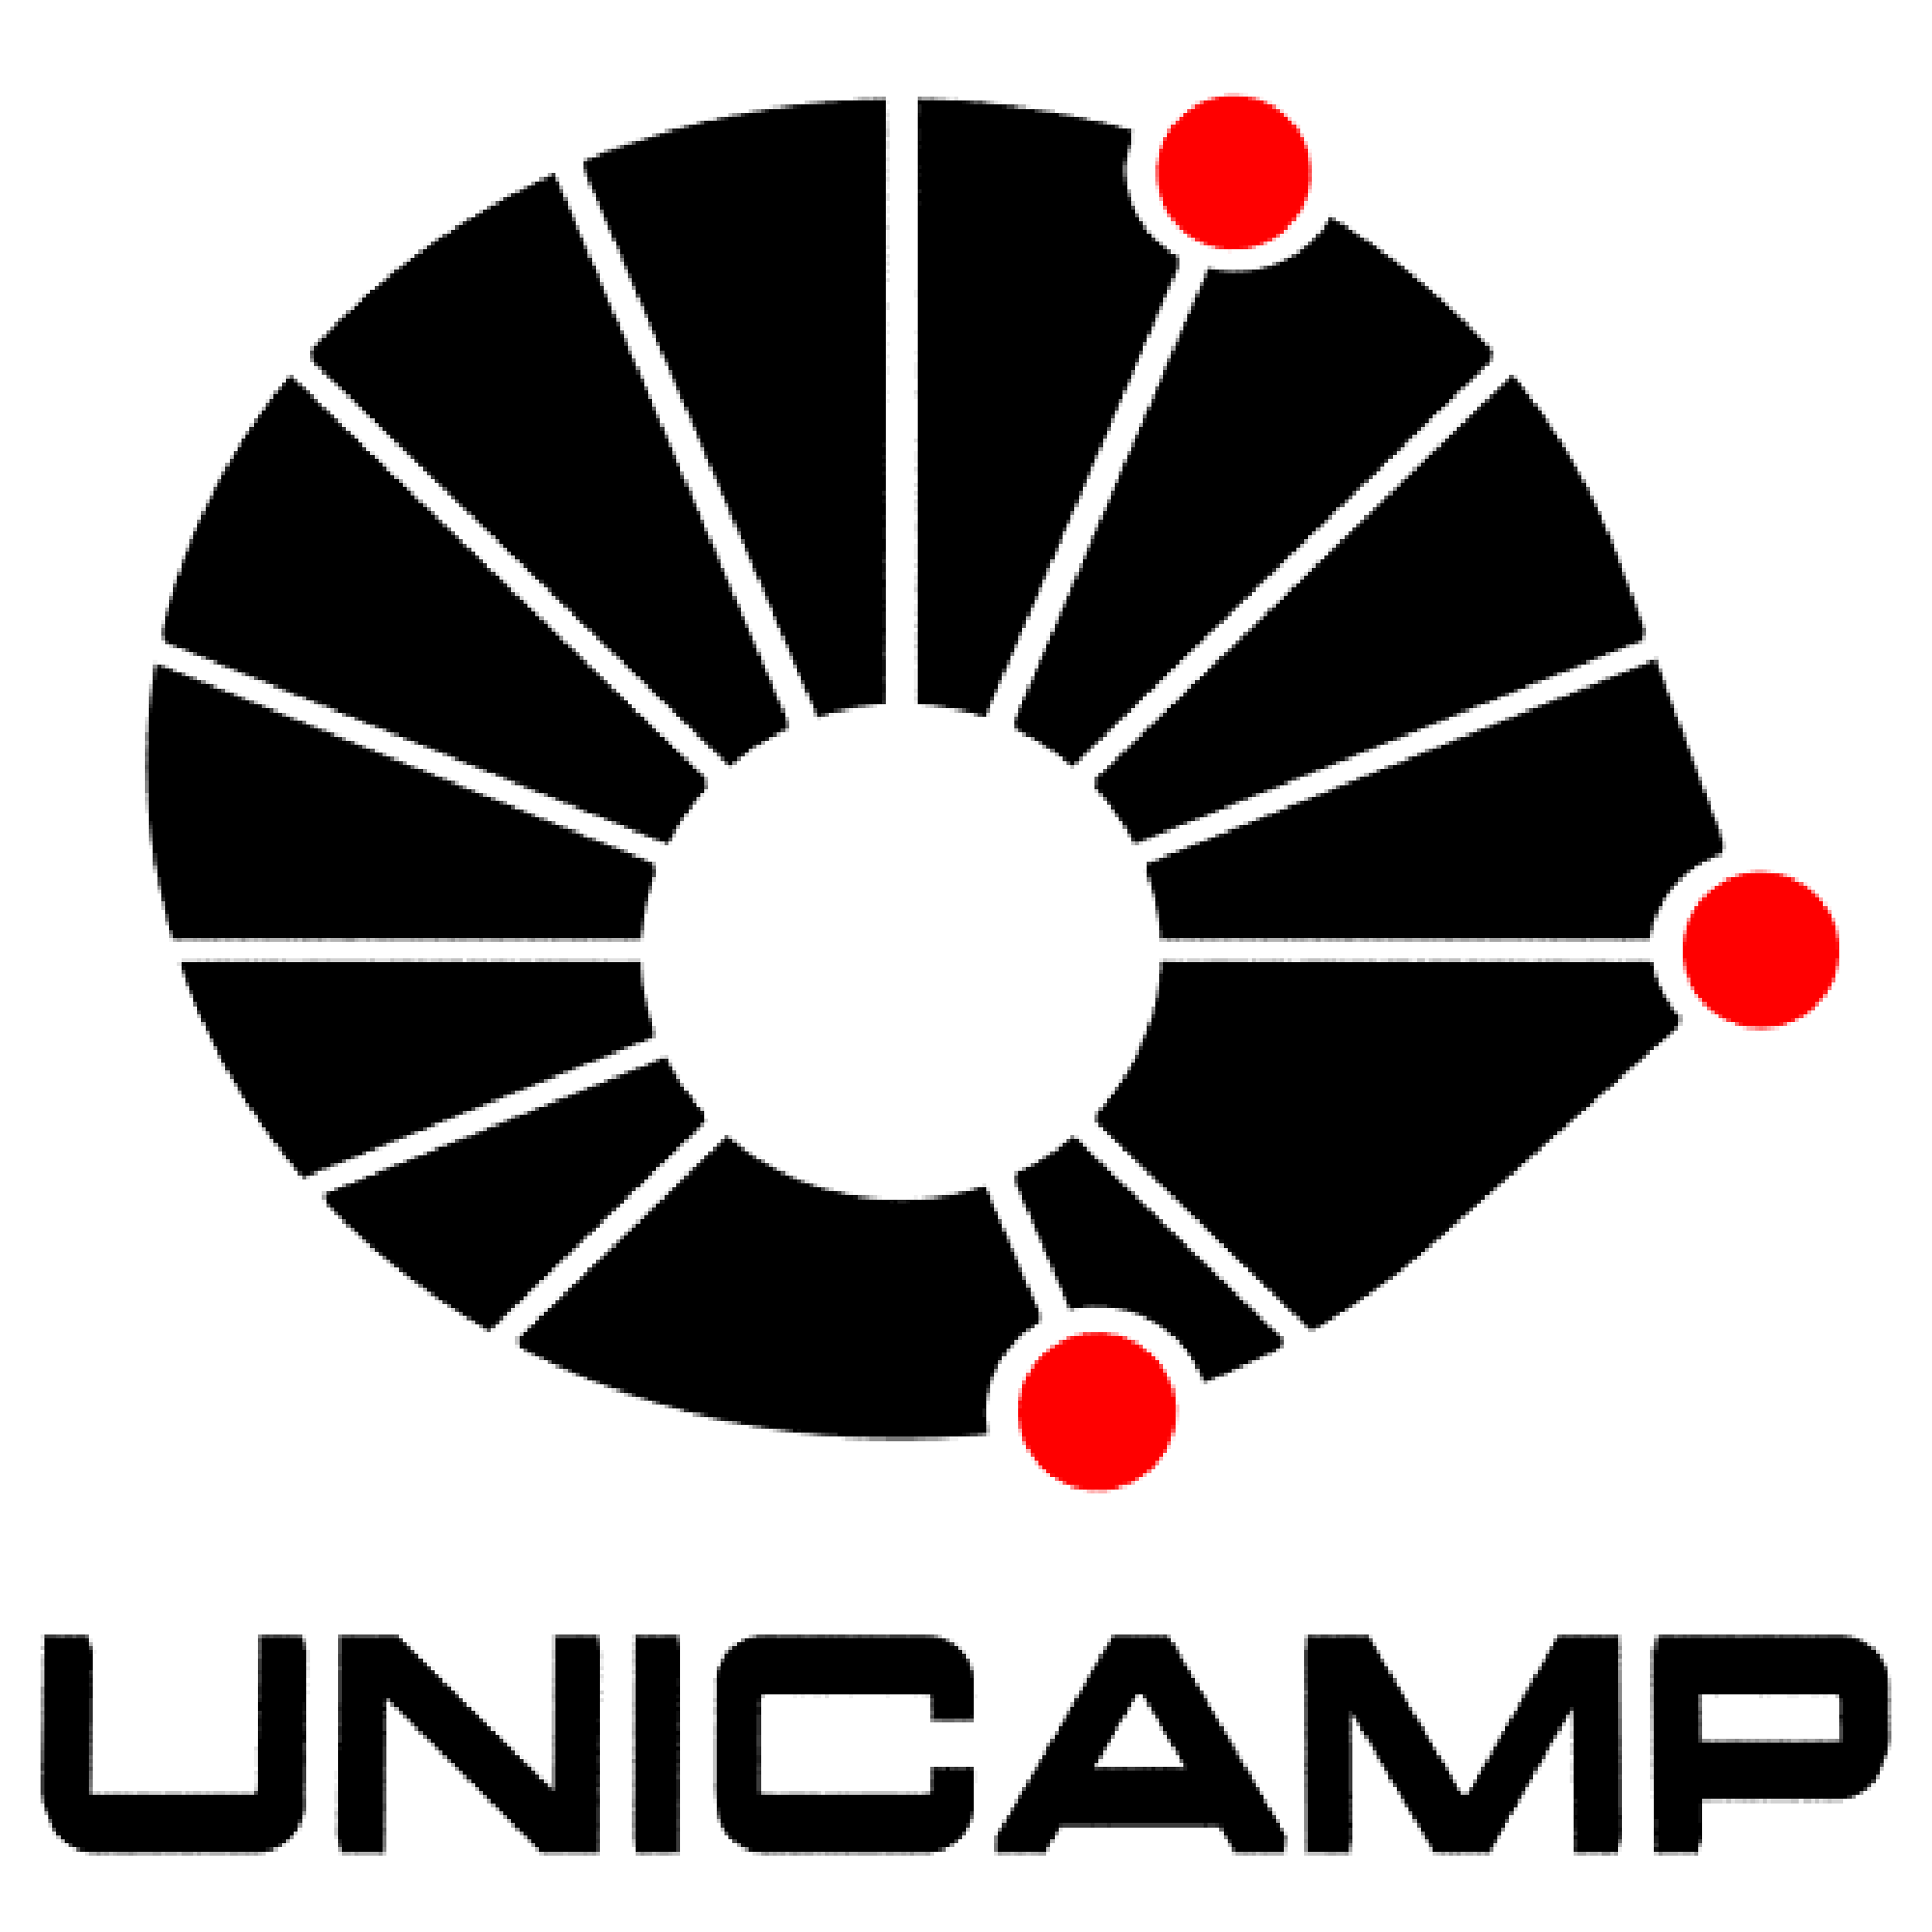
\includegraphics[scale=0.2]{images/logo-unicamp.png}}
% \caption[Shorter figure caption]{Figure Caption caption caption caption
%   caption caption caption caption caption caption caption caption caption
%   caption caption caption caption caption caption caption caption caption
%   caption caption.}
% \label{f:label1}
% \end{figure}
